\documentclass[a4paper,14pt]{extarticle}

\usepackage[a4paper,top=20mm,bottom=20mm,left=30mm,right=10mm]{geometry}
\usepackage[T1,T2A]{fontenc}
\usepackage[utf8]{inputenc}
\usepackage[russian]{babel}
\usepackage{indentfirst}
\usepackage{titlesec}
\usepackage{graphicx}
\usepackage{verbatim}
\usepackage{fancyvrb}

\renewcommand{\baselinestretch}{1.3}
\titleformat{\section}{\normalsize\bfseries}{\thesection}{1em}{}
\titleformat{\subsection}{\normalsize\bfseries}{\thesection}{1em}{}
\setlength{\parindent}{12.5mm}

\begin{document}

	\newpage\thispagestyle{empty}
	\begin{center}
		\MakeUppercase{
			Министерство науки и высшего образования Российской Федерации\\
			Федеральное государственное бюджетное образовательное учреждение высшего образования\\
			<<Вятский Государственный Университет>>\\
		}
		Институт математики и информационных систем\\
		Факультет автоматики и вычислительной техники\\
		Кафедра электронных вычислительных машин
	\end{center}
	\vfill
	
	\begin{center}
		Отчет по лабораторной работе №4\\
		по дисциплине\\
		<<Программирование>>\\
	\end{center}
	\vfill
	
	\noindent
	\begin{tabular}{ll}
		Выполнил студент гр. ИВТб-1301-05-00 \hspace{5mm} &
		\rule[-1mm]{25mm}{0.10mm}\,/Макаров С.А./\\
		
		Руководитель зав. кафедры ЭВМ & \rule[-1mm]{25mm}{0.10mm}\,/Долженкова М.Л./\\
	\end{tabular}
	
	\vfill
	\begin{center}
		Киров 2024
	\end{center}
	
	\newpage
	\section*{Цель}
	Цель лабораторной работы: освоить навык создания структур данных на статических массивах их использование в решении задач.
	
	\section*{Задание}
	Даны действительные числа $a_1$, $s_2$, ..., $a_{2n}$ (n >= 2, заранее неизвестно и вводится с клавиатуры). Вычислите: max(min($a_1$, $a_{2n}$), min($a_3$, $a_{2n-2}$), ..., min($a_{2n-1}$, $a_2$)).
	
	\section*{Решение}
	Для решения данной необходимо использовать двунаправленный список, так как по условию задачи необходимо двигаться в обе стороны списка и среди них искать минимальное число попарно.\\
	\indent К преимуществам двунаправленного списка в сравнении с односвязным списком относятся возможность двигаться в как с начала списка, так и с конца, что позволяет быстрее получать доступ к элементам списка в зависимости от их расположения.\\
	
	\begin{figure}[h]
		\centering
		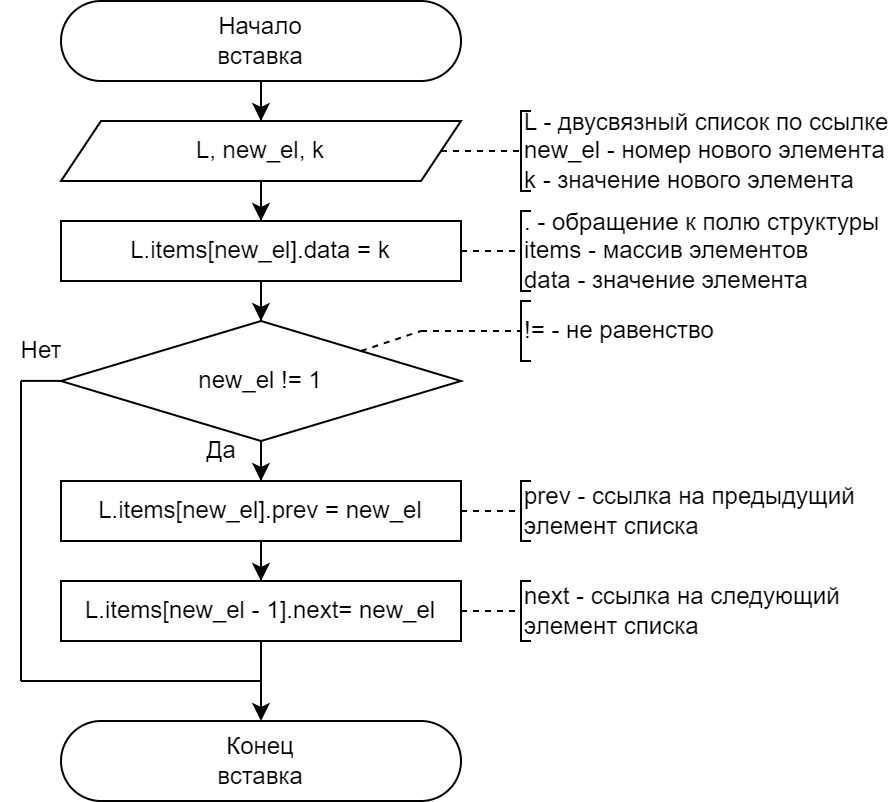
\includegraphics[width=0.56\linewidth]{images/s-1}
	\end{figure}
	\begin{center}
		Рисунок 1 – Подпрограмма <<Вставка>>
	\end{center}
	
	\pagebreak
	\begin{figure}[h]
		\centering
		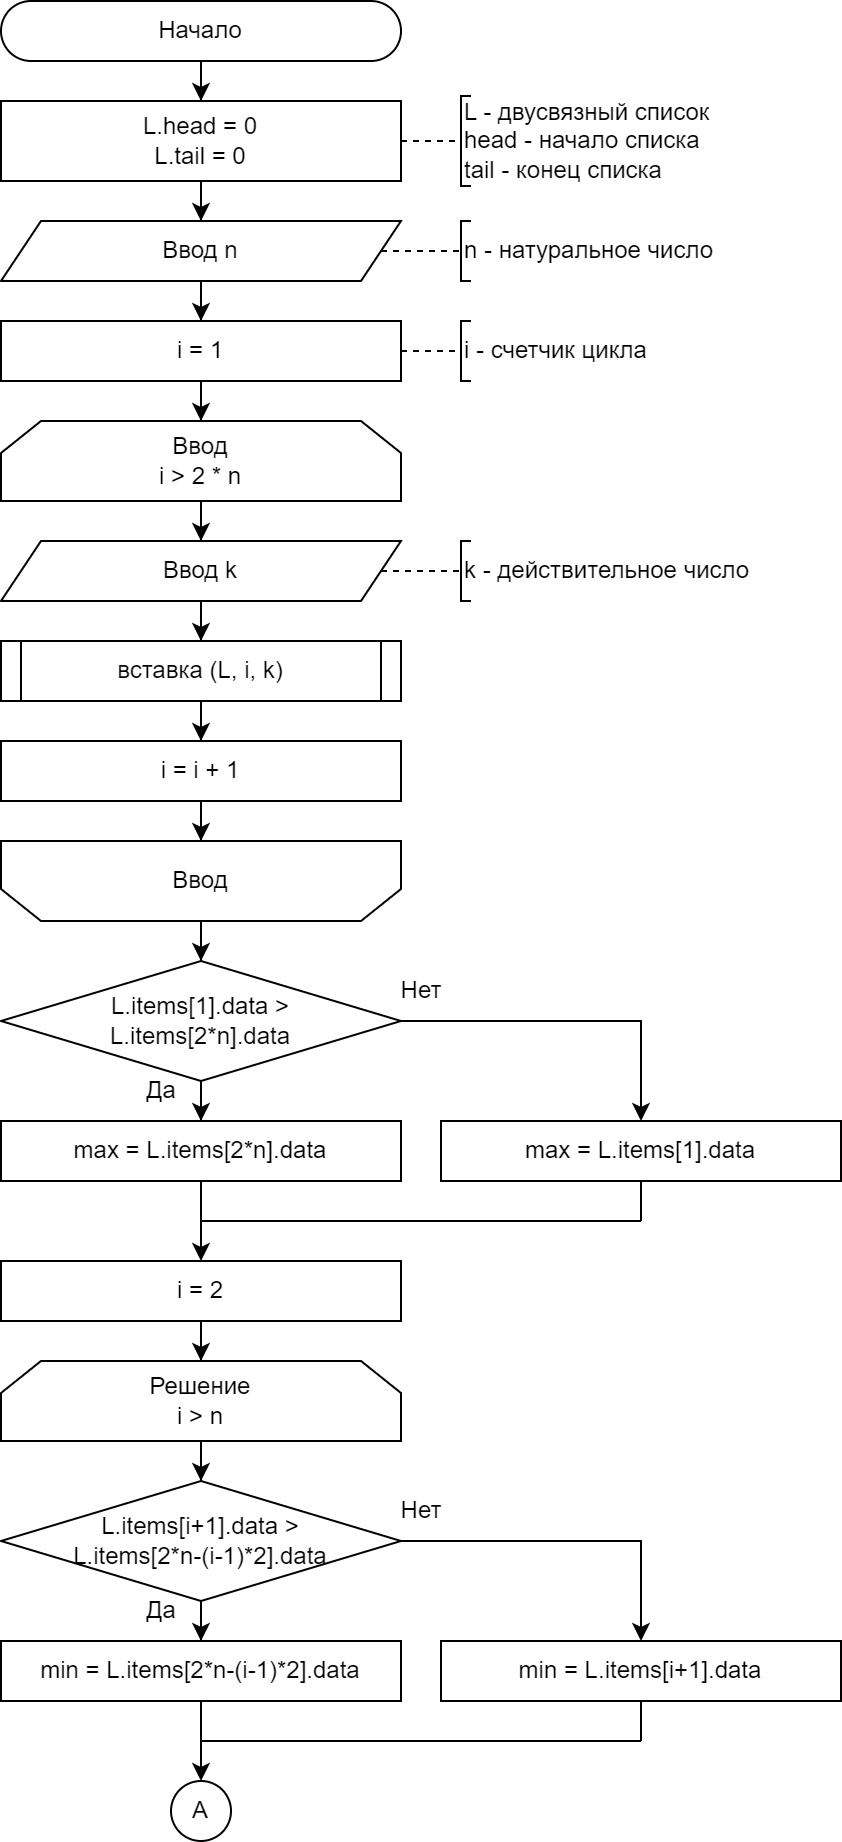
\includegraphics[width=0.538\linewidth]{images/s-2}
	\end{figure}
	\begin{center}
		Рисунок 2 – Схема алгоритма программы
	\end{center}
	
	\pagebreak
	\begin{figure}[h]
	\centering
		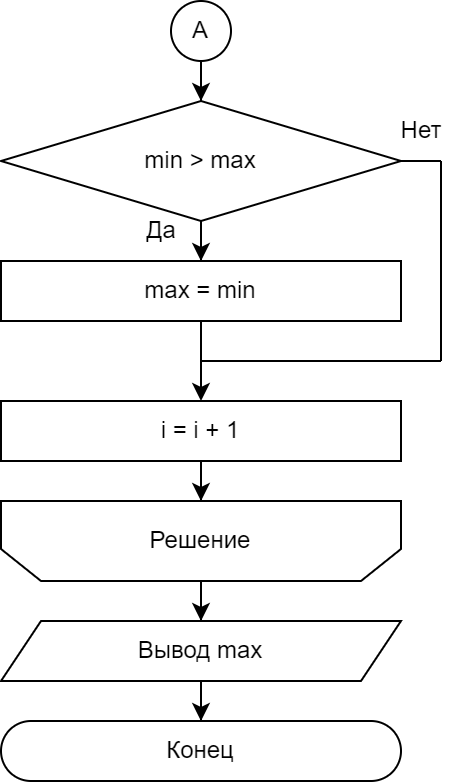
\includegraphics[width=0.4\linewidth]{images/s-3}
	\end{figure}
	\begin{center}
		Рисунок 3 – Продолжение схемы алгоритма
	\end{center}
	
	\begin{Verbatim}[tabsize=2]
program solution;

type
	item = record
		data: integer;
		next, prev:byte;
	end;

	list = record
		items:array[1..100] of item;
		head, tail:byte;
	end;
var
	n, k, i, max, min:integer;
	L:list;

procedure push(var L:list; new_el:integer; k:integer);
begin
	L.items[new_el].data := k;
	
	if new_el <> 1 then
	begin
		L.items[new_el].prev := new_el;
		L.items[new_el - 1].next := new_el;
	end;
end;

begin
	L.head := 0;
	L.tail := 0;
	readln(n);
	for i := 1 to 2 * n do
	begin
		read(k);
		push(L, i, k);
	end;
	
	if L.items[1].data > L.items[2 * n].data then
		max := L.items[2 * n].data
	else
		max := L.items[1].data;
	
	for i := 2 to n do
	begin
	if L.items[i + 1].data > L.items[2 * n - (i - 1) * 2].data then
		min := L.items[2 * n - (i - 1) * 2].data
	else
		min := L.items[i + 1].data;
	
	if min > max then
		max := min;
	end;
	
	writeln(max);
end.
	\end{Verbatim}
	
	\section*{Вывод}
	В ходе выполнения лабораторной работы удалось освоить и реализовать такую структуру данных как двунаправленный список путем решения предложенной задачи.

\end{document}